%
% Niniejszy plik stanowi przykład formatowania pracy magisterskiej na
% Wydziale MIM UW.  Szkielet użytych poleceń można wykorzystywać do
% woli, np. formatujac wlasna prace.
%
% Zawartosc merytoryczna stanowi oryginalnosiagniecie
% naukowosciowe Marcina Wolinskiego.  Wszelkie prawa zastrzeżone.
%
% Copyright (c) 2001 by Marcin Woliński <M.Wolinski@gust.org.pl>
% Poprawki spowodowane zmianami przepisów - Marcin Szczuka, 1.10.2004
% Poprawki spowodowane zmianami przepisow i ujednolicenie 
% - Seweryn Karłowicz, 05.05.2006
% Dodanie wielu autorów i tłumaczenia na angielski - Kuba Pochrybniak, 29.11.2016

% dodaj opcję [licencjacka] dla pracy licencjackiej
% dodaj opcję [en] dla wersji angielskiej (mogą być obie: [licencjacka,en])
\documentclass[licencjacka]{style}


% Dane magistranta:
%\autor{Imię Nazwisko}{123456}


% Dane magistrantów:
\autor{Magdalena Grabowska}{372701}
\autori{Michał Kukuła}{371127}
\autorii{Klaudia Laks}{371151}
\autoriii{Przemysław Perkowski}{371308}
%\autoriv{Autor nr Cztery}{432145}
%\autorv{Autor nr Pięć}{342011}

\title{Miejsca Obsługi Podróżnych}


\tytulang{Parking places at rest areas on highways and expressways in Poland}

%kierunek: 
% - matematyka, informacyka, ...
% - Mathematics, Computer Science, ...
\kierunek{informatyka}

% informatyka - nie okreslamy zakresu (opcja zakomentowana)
% matematyka - zakres moze pozostac nieokreslony,
% a jesli ma byc okreslony dla pracy mgr,
% to przyjmuje jedna z wartosci:
% {metod matematycznych w finansach}
% {metod matematycznych w ubezpieczeniach}
% {matematyki stosowanej}
% {nauczania matematyki}
% Dla pracy licencjackiej mamy natomiast
% mozliwosc wpisania takiej wartosci zakresu:
% {Jednoczesnych Studiow Ekonomiczno--Matematycznych}

% \zakres{Tu wpisac, jesli trzeba, jedna z opcji podanych wyzej}

% Praca wykonana pod kierunkiem:
% (podać tytuł/stopień imię i nazwisko opiekuna
% Instytut
% ew. Wydział ew. Uczelnia (jeżeli nie MIM UW))
\opiekun{dr. hab. Aleksego Schuberta\\
  }

% miesiąc i~rok:
\date{Czerwiec 2018}

%Podać dziedzinę wg klasyfikacji Socrates-Erasmus:
\dziedzina{ 
%11.0 Matematyka, Informatyka:\\ 
%11.1 Matematyka\\ 
%11.2 Statystyka\\ 
11.3 Informatyka\\ 
%11.4 Sztuczna inteligencja\\ 
%11.5 Nauki aktuarialne\\
%11.9 Inne nauki matematyczne i informatyczne
}

%TODO Tu trzeba wpisać jakieś numerki ale nie umiem ich znaleźć.
%Klasyfikacja tematyczna wedlug AMS (matematyka) lub ACM (informatyka)
\klasyfikacja{D. Software \\ \\}


%TODO napisać jakieś
%Słowa kluczowe:
\keywords{symulacja, wizualizacja, Miejsce Obsługi Podróżnych, miejsce parkingowe, aplikacja okienkowa, aplikacja mobilna, strona internetowa, zajętość miejsc parkingowych, natężenie ruchu}

% Tu jest dobre miejsce na Twoje własne makra i~środowiska:
\newtheorem{defi}{Definicja}[section]

% koniec definicji

\usepackage{graphicx}
\usepackage{hyperref}
\begin{document}

\maketitle

%tu idzie streszczenie na strone poczatkowa
\begin{abstract}
  W~pracy opisano implementację systemu dotyczącego Miejsc Obsługi Podróżnych
  przy autostradach i~drogach ekspresowych w Polsce. Podstawowe składowe tego
  systemu to aplikacje Mopnik i~Mopsim. Są one aplikacjami okienkowymi
  korzystającymi ze wspólnego interfejsu graficznego. Służą do~przeprowadzania
  krótko- i~długoterminowych predykcji ruchu na drogach oraz zajętości miejsc
  parkingowych na~Miejscach Obsługi Podróżnych. Pozostałe dwie części to
  aplikacja mobilna oraz strona internetowa przeznaczone dla kierowców
  poruszających się po drogach. Informują one o~zajętości miejsc parkingowych
  na każdym MOPie w danym momencie oraz predyckji ich zajętości w niedalekiej
  przyszłości.  
  %TODO napisać coś jak będzie co streszczać 
\end{abstract}

\tableofcontents
%\listoffigures
%\listoftables

\chapter*{Słowniczek}\label{r:pojecia}
\addcontentsline{toc}{chapter}{Słowniczek}

\begin{defi}\label{GDDKiA}
  \emph{GDDKiA} - Generalna Dyrekcja Dróg Krajowych i Autostrad.
\end{defi}

\begin{defi}\label{MOP}
  \emph{MOP} - Miejsce Obsługi Podróżnych.
\end{defi}

\begin{defi}\label{SDR}
  \emph{SDR} - Średniodobowe natężenie ruchu.
\end{defi}

\begin{defi}\label{GUI}
  \emph{GUI} - Graficzny interfejs użytkownika.
\end{defi}

\begin{defi}\label{OSM}
  \emph{OSM} - Serwis OpenStreetMap (http://openstreetmap.org).
\end{defi}

\chapter{Wprowadzenie}

\section{Rozwój sieci drogowej w Polsce}
Jeszcze pod koniec XX w. w Polsce znajdowało się zaledwie ok. 500km autostrad i dróg ekspresowych. Pomimo licznych planów rozwojowych, które przyjmowane były w okresie PRL i pierwszych latach III RP, większość dróg budowana była z dużymi opóźnieniami, a niektórych odcinków nie realizowano wcale.\newline
Dopiero przyjęty pod koniec lat 90. program budowy sieci autostrad i dróg ekspresowych w Polsce, mimo wielu modyfikacji jest na bieżąco realizowany. Jako przyczyny\cite{siec-drogowa-IIIrp} przyspieszenia budowy dróg szybkiego ruchu w Polsce wymienia się między innymi: duże zainteresowanie problemem, wzrost liczby pojazdów, dotacje z europejskiego Funduszu Spójności, a także dotacje Unii Europejskiej. Dodatkowym impulsem mobilizującym instytucje rządowe do przyspieszenia prac w tym kierunku stało się przyznanie organizacji Euro 2012 Polsce i Ukrainie.\newline
\begin{figure}[h]
\caption{Rozwój sieci dróg ekspresowych i autostrad w Polsce na początku XX w.}
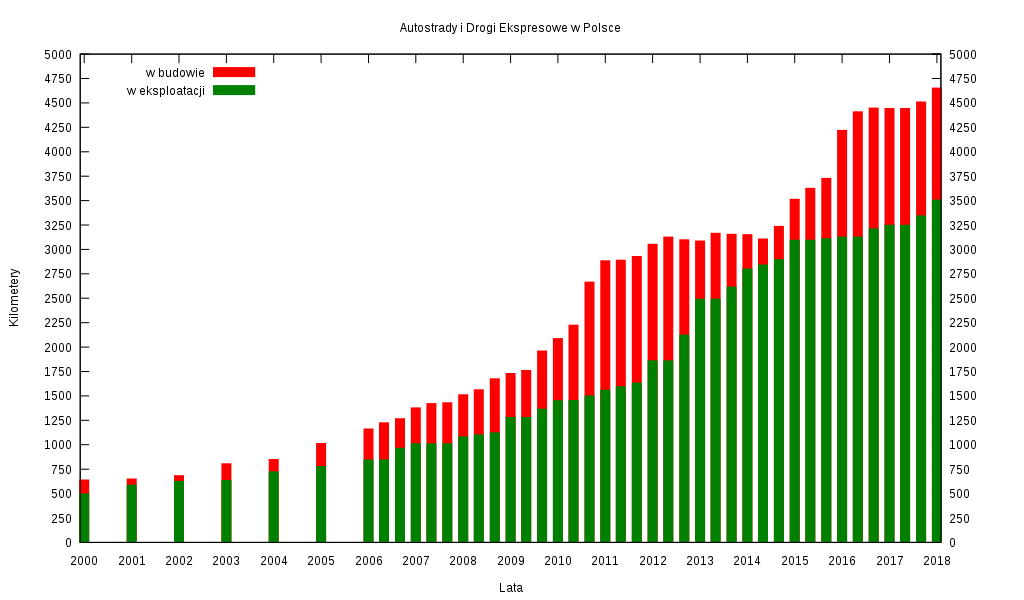
\includegraphics[width=\textwidth]{images/1024px-PL-Motorways.png}
\end{figure} \newline
Ostatnie lata to okres szczególnie intensywnego rozwoju sieci drogowej w Polsce. Budowa infrastruktury wiąże się również z potrzebą zapewnienia podróżnym bezpieczeństwa i komfortu.
\begin{figure}[h]
\caption{Sieć autostrad i dróg ekspresowych w Polsce (styczeń 2018r.). Na zielono - odcinki zrealizowane, na czerwono - odcinki w budowie, na szaro - odcinki planowane.}
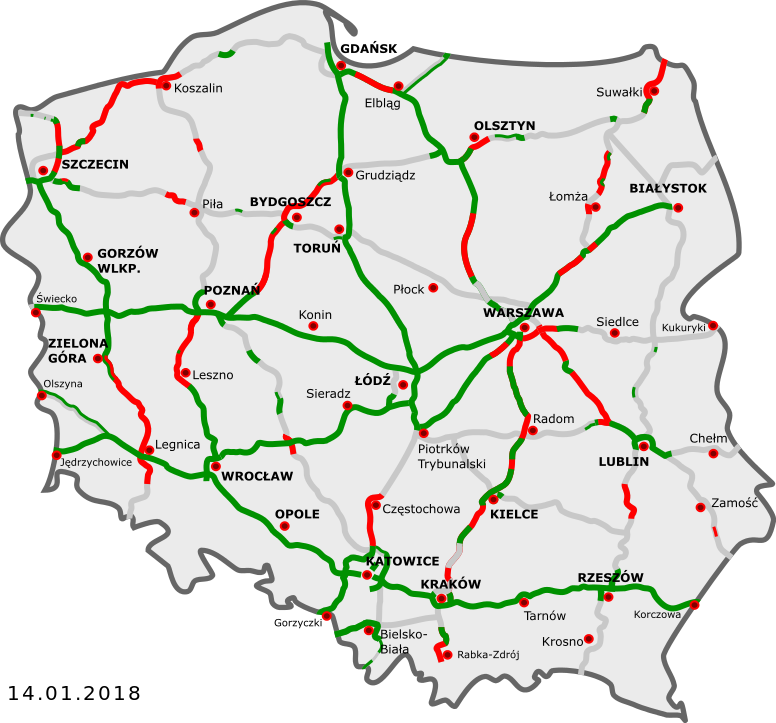
\includegraphics[width=\textwidth]{images/2018.png}
\end{figure}

\section{Miejsca Obsługi Podróżnych}
Miejsce Obsługi Podróżnych (\textbf{MOP}) to teren wydzielony w pasie drogowym (w bliskim sąsiedztwie drogi), wyposażony w parking oraz w infrastrukturę zapewniającą komfort i odpoczynek podróżnym\cite{gddkia-mop}. MOP-y powstają tylko przy autostradach i drogach ekspresowych.\newline
MOP-y w Polsce dzielimy na trzy kategorie:
\begin{enumerate}
    \item \textbf{MOP kategorii I} - o funkcji wypoczynkowej, wyposażony w stanowiska postojowe (parking), jezdnie manewrowe, urządzenia wypoczynkowe, sanitarne i oświetlenie; dopuszcza się wyposażenie w obiekty małej gastronomii.
    \item \textbf{MOP kategorii II} - - o funkcji wypoczynkowo-usługowej, wyposażony w obiekty, o których mowa
w punkcie 1., oraz w stację paliw, stanowiska obsługi pojazdów, obiekty gastronomiczno-handlowe, punkty informacji turystycznej.
    \item \textbf{MOP kategorii III} - - o funkcji wypoczynkowej i usługowej, wyposażony w obiekty, o których mowa w punkcie 2., obiekty noclegowe oraz inne obiekty handlowo-usługowe w zależności od potrzeb.
\end{enumerate}
\begin{figure}[h]
\caption{Aktualne (styczeń 2018r.) pozycje MOP-ów w Polsce (na niebiesko). MOP-y planowane (na czerwono).}
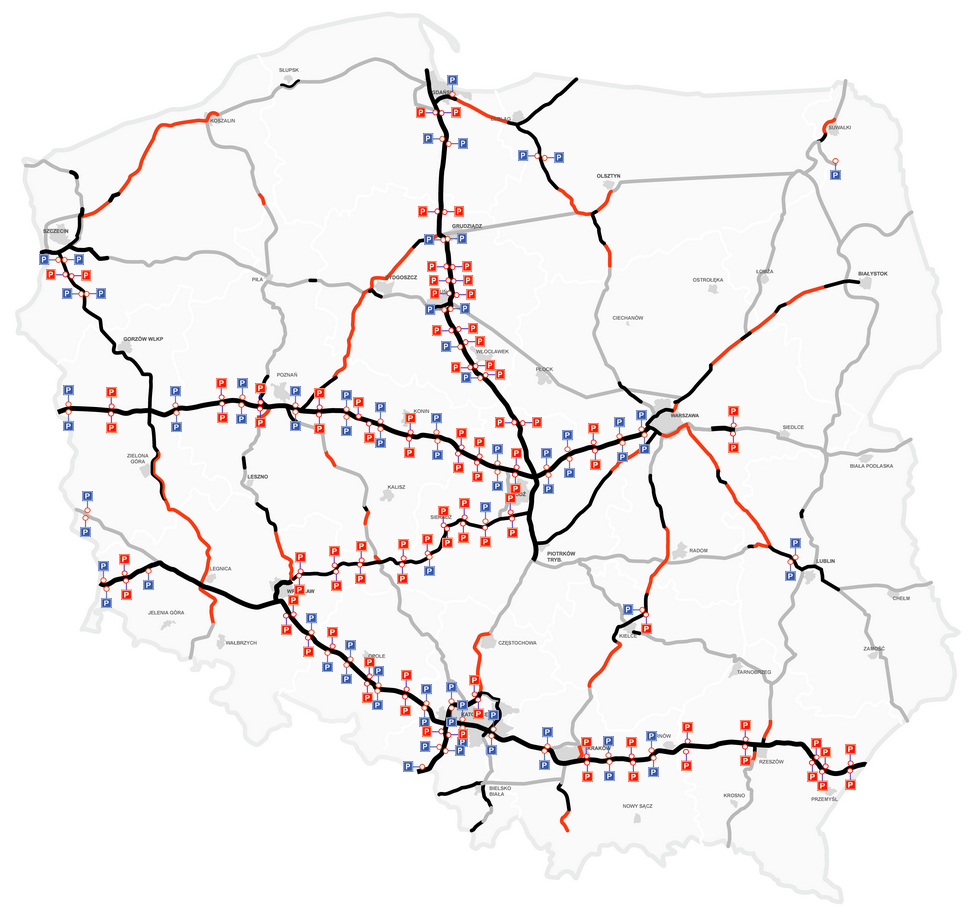
\includegraphics[width=\textwidth]{images/mopymap.png}
\end{figure}

\section{Problemy związane z budową MOP-ów}
Intensywny rozwój sieci drogowej, a co za tym idzie również szybki wzrost liczby MOP-ów w Polsce stwarza szereg problemów z nimi związanych:
\begin{enumerate}
    \item \textbf{Problemy administracyjno-prawne} - GDDKIA systematycznie prowadzi kolejne przetargi na dzierżawę MOP zlokalizowanych zarówno przy autostradach jak i drogach ekspresowych. Dzierżawa nieruchomości MOP generuje przychody, które systematycznie zasilają budżet Krajowego Funduszu Drogowego. Nieatrakcyjne warunki umowy lub lokalizacja punktu mogą zniechęcać potencjalnych najemców.
    \item \textbf{Lokalizacja MOP-ów} - efektywne rozmieszczenie MOP-ów powinno uwzględniać takie parametry jak: odległość od najbliższych MOP-ów, natężenie odcinka drogi, odległość od węzłów komunikacyjnych.
    \item \textbf{Liczba miejsc parkingowych i ich układ} - MOP-y powinny dysponować taką liczbą miejsc parkingowych, by zapewnić możliwość odpoczynku podróżującym także w warunkach wzmożonego ruchu. Rozmieszczenie miejsc parkingowych powinno zapewnić kierowcom komfort podczas poruszania się pojazdem na terenie punktu.
\end{enumerate}

\section{Symulacja ruchu drogowego w Polsce}
Efektywne rozmieszczenie coraz większej liczby MOP-ów jest jednym z głównych wyzwań, stojących przed planistami dróg. Powinno ono uwzględniać wszystkie kwestie poruszone w poprzednim rozdziale. Jednak rozwój sieci drogowej w Polsce na niespotykaną wcześniej skalę sprawia, że zadanie to jest coraz trudniejsze. Może się okazać, że dane dotyczące natężenia ruchu na danym odcinku drogi, odległości od najbliższych MOP-ów czy węzłów komunikacyjnych są niewystarczające i trudno na ich podstawie określić wykorzystanie MOP-a w okresach wzmożonego ruchu sezonowego lub w przyszłości, wraz z dalszym rozwojem infrastruktury drogowej. Przydatnymi danymi, wykorzystywanymi w modelowaniu ruchu drogowego, są macierze podróży, określające liczbę pojazdów poruszających się pomiędzy danymi parami punktów w zadanym okresie. Planista dróg, wyposażony w macierze podróży, chciałby na ich podstawie wiedzieć:
\begin{enumerate}
	\item Jakie jest natężenie ruchu na poszczególnych odcinkach drogi?
	\item Jak dodanie lub usunięcie (np. w wyniku tymczasowego zatrzymania ruchu) odcinka drogi wpłynie na to natężenie?
	\item Jaka część podróżnych, jadąca danym odcinkiem drogi, chciałaby skorzystać z MOP-a?
\end{enumerate}
Pomocny w przeprowadzeniu tej analizy może okazać się \textbf{MOPSim} - program komputerowy symulujący ruch pojazdów na
sieci dróg krajowych i autostrad w Polsce.

\section{coś o mopniku}


\section{Zajętość MOP-ów i dostępne usługi}
Jednym ze wspomnianych wcześniej problemów związanych z budową MOP-ów jest dobór odpowiedniej liczby miejsc parkingowych. Dodatkowo, miejsca te należy odpowiednio podzielić pomiędzy różne typy pojazdów: samochody osobowe, samochody ciężarowe, autobusy, pojazdy przewożące substancje niebezpieczne itd. Podróżni mają też różne potrzeby związane z postojem - od szybkiego zatankowania samochodu, przez obiad z rodziną na świeżym powietrzu, do spędzenia nocy w kabinie. \newline Aktualnie informację o znajdujących się na MOP-ie usługach można uzyskać ze znaków informacyjnych umieszczonych kilka kilometrów przed zjazdem. Jednak takie oznaczenia nie odpowiadają na kilka ważnych pytań, które możemy mieć na dowolnym etapie podróży:
\begin{enumerate}
	\item Za ile kilometrów znajduje się najbliższa stacja benzynowa? 
	\item Czy starczy mi paliwa do następnej, ponieważ tutaj jest duża kolejka?
	\item Czy na tym MOP-ie jest monitoring?
	\item Czy na tym MOP-ie są wolne miejsca parkingowe? (ten problem jest ważniejszy z punktu widzenia kierowców pojazdów wielkogabarytowych)
	\item Jaka będzie zajętość miejsc parkingowych za godzinę?
\end{enumerate}
Odpowiedzią na te pytania będzie \textbf{MOPSIK} (MOP - System Informowania Kierowców) - aplikacja mobilna i strona internetowa.

\chapter{Mopnik}\label{r:mopnik}

\section{Podejście wprost}

Najprostszym sposobem wykonania blabalizy jest siłowe przeszukanie
całej przestrzeni rozwiązań.  Jednak, jak łatwo wyliczyć, rozmiar
przestrzeni rozwiązań rośnie wykładniczo z~liczbą fetorów bazowych.
Tak więc przegląd wszystkich rozwiązań sprawdza się jedynie dla bardzo
prostych przestrzeni lamblialnych.  Oznacza to, że taka metoda ma
niewielkie znaczenie praktyczne --- w~typowym przypadku z~życia trzeba
rozważać przestrzenie lamblialne wymiaru rzędu 1000.

W~literaturze można znaleźć kilka prób opracowania heurystyk dla
problemu blabalizy (por. \cite{heu}).  Korzystając z~heurystyk daje
się z~pewnym trudem dokonać blabalizy w~przestrzeni o~np.~500 fetorach
bazowych.  Należy jednak pamiętać, że heurystyka nie daje gwarancji
znalezienia najlepszego rozwiązania.  Fifak w~pracy~\cite{ff-sr}
podaje, jak dla dowolnie zadanej funkcji oceniającej skonstruować
dane, dla których rozwiązanie wygenerowane przez algorytm heurystyczny
jest dowolnie odległe od rzeczywistego.

\section{Metody wykorzystujące teorię Głombaskiego}

Teoria Głombaskiego (zob.~\cite{grglo}) dostarcza eleganckiego
narzędzia opisu przejścia do przestrzeni $\Lambda^{\nabla}$.
Wystarczy mianowicie przedstawić fetory bazowe wyjściowej przestrzeni
lamblialnej w~nieskończonej bazie tak zwanych wyższych aromatów.
(Formalną definicję tego pojęcia przedstawię w~rozdziale poświęconym
teorii Fifaka).  Podstawową cechą wyższych aromatów jest ulotność.  To
zaś oznacza, że odpowiednio dobierając współczynniki przejścia do
przestrzeni wyższych aromatów można zagwarantować dowolną z~góry
zadaną dokładność przybliżonego rozwiązania problemu blabalizy.

Oczywiście ze względu na nieskończony wymiar przestrzeni wyższych
aromatów koszt poszukiwania współczynników blabalizy jest liniowy ze
względu na wymiar wyjściowej przestrzeni lamblialnej.

\section{Metody wykorzystujące własności fetorów $\sigma$}

Najchętniej wykorzystywaną przestrzenią wyższych aromatów jest
przestrzeń fetorów~$\sigma$.  Fetory $\sigma$ dają szczególnie prostą
bazę podprzestrzeni widłowej.  Wiąże się to z~faktem, że w~tym przypadku
fetory harmoniczne wyższych rzędów są pomijalne (rzędu $2^{-t^3}$,
gdzie $t$ jest wymiarem wyjściowej przestrzeni lamblialnej).

Niestety z~fetorami $\sigma$ wiąże się też przykre ograniczenie: można
wykazać (zob.~\cite[s. 374]{ff-sr}), że dla dowolnie dobranej bazy
w~podprzestrzeni widłowej istnieje ograniczenie dolne w~metryce sierpa
na odległość rzutu dokładnego rozwiązania problemu blabalizy na
podprzestrzeń widłową.  Ponieważ rzut ten stanowi najlepsze
przybliżone rozwiązanie, jakie można osiągnąć nie naruszając aksjomatu
reperkusatywności, więc istnieje pewien nieprzekraczalny próg
dokładności dla blabalizy wykonanej przez przejście do przestrzeni
fetorów $\sigma$.  Wartość retroinicjalną tego progu nazywa się
\textit{reziduum blabicznym}.

\chapter{Mopsim}\label{r:mopsim}

Głównym odkryciem Fifaka jest, że fetor suprakowariantny może
gryzmolizować dowolny ideał w~podprzestrzeni widłowej przestrzeni
lamblialnej funkcji Rozkoszy.

Udowodnienie tego faktu wymagało wykorzystania twierdzeń pochodzących
z~kilku niezależnych teorii matematycznych (zob. na przykład:
\cite{russell,spyrpt,JR,beaman,hopp,srinis}).  Jednym z~filarów
dowodu jest teoria odwzorowań owalnych Leukocyta (zob.~\cite{leuk}).

Znaczenie twierdzenia Fifaka dla problemu blabalizy polega na tym, że
znając retroizotonalne współczynniki dla klatek Rozkoszy można
przeprowadzić fetory bazowe na dwie nieskończone bazy fetorów $\sigma$
w~przestrzeni $K_7$ i~fetorów $\rho$ w~odpowiedniej
quasi-quasi-przestrzeni równoległej (zob.~\cite{hopp}).  Zasadnicza
różnica w~stosunku do innych metod blabalizy polega na tym, że
przedstawienie to jest dokładne.

\chapter{Dokumentacja użytkowa i~opis implementacji}\label{r:impl}

Program przygotowany dla systemu operacyjnego M\$ Windows uruchamia
się energicznym dwumlaskiem na jego ikonce w~folderze
\verb+\\FIDO\FOO\BLABA+.  Następnie kolistym ruchem ręki należy
naprowadzić kursor na menu \texttt{Blabaliza} i~uaktywnić pozycję
\texttt{Otwórz plik}.  Po wybraniu pliku i~zatwierdzeniu wyboru
przyciskiem \texttt{OK} rozpocznie się proces blabalizy.  Wyniki
zostaną zapisane w~pliku o~nazwie \texttt{99-1a.tx.43} w~bieżącym
folderze.

\chapter{Aplikacja mobilna i strona internetowa}\label{r:apka} 

\chapter{Podsumowanie}

W~pracy przedstawiono pierwszą efektywną implementację blabalizatora
różnicowego.  Umiejętność wykonania blabalizy numerycznej dla danych
,,z życia'' stanowi dla blabalii fetorycznej podobny przełom, jak dla
innych dziedzin wiedzy stanowiło ogłoszenie teorii Mikołaja Kopernika
i~Gryzybór Głombaskiego.  Z~pewnością w~rozpocznynającym się XXI wieku
będziemy obserwować rozkwit blabalii fetorycznej.

Trudno przewidzieć wszystkie nowe możliwości, ale te co bardziej
oczywiste można wskazać już teraz.  Są to:
\begin{itemize}
\item degryzmolizacja wieńców telecentrycznych,
\item realizacja zimnej reakcji lambliarnej,
\item loty celulityczne,
\item dokładne obliczenie wieku Wszechświata.
\end{itemize}

\section{Perspektywy wykorzystania w~przemyśle}

Ze względu na znaczenie strategiczne wyników pracy ten punkt uległ
utajnieniu.

\appendix

\chapter{Główna pętla programu zapisana w~języku T\=oFoo}

\begin{verbatim}
[[foo]{,}[[a3,(([(,),{[[]]}]),
  [1; [{,13},[[[11],11],231]]].
  [13;[!xz]].
  [42;[{,x},[[2],{'a'},14]]].
  [br;[XQ*10]].
 ), 2q, for, [1,]2, [..].[7]{x}],[(((,[[1{{123,},},;.112]],
        else 42;
   . 'b'.. '9', [[13141],{13414}], 11),
 [1; [[134,sigma],22]].
 [2; [[rho,-],11]].
 )[14].
 ), {1234}],]. [map [cc], 1, 22]. [rho x 1]. {22; [22]},
       dd.
 [11; sigma].
        ss.4.c.q.42.b.ll.ls.chmod.aux.rm.foo;
 [112.34; rho];
        001110101010101010101010101010101111101001@
 [22%f4].
 cq. rep. else 7;
 ]. hlt
\end{verbatim}

\chapter{Przykładowe dane wejściowe algorytmu}

\begin{center}
  \begin{tabular}{rrr}
    $\alpha$ & $\beta$ & $\gamma_7$ \\
    901384 & 13784 & 1341\\
    68746546 & 13498& 09165\\
    918324719& 1789 & 1310 \\
    9089 & 91032874& 1873 \\
    1 & 9187 & 19032874193 \\
    90143 & 01938 & 0193284 \\
    309132 & $-1349$ & $-149089088$ \\
    0202122 & 1234132 & 918324098 \\
    11234 & $-109234$ & 1934 \\
  \end{tabular}
\end{center}

\chapter{Przykładowe wyniki blabalizy
    (ze~współczynnikami~$\sigma$-$\rho$)}

\begin{center}
  \begin{tabular}{lrrrr}
    & Współczynniki \\
    & Głombaskiego & $\rho$ & $\sigma$ & $\sigma$-$\rho$\\
    $\gamma_{0}$ & 1,331 & 2,01 & 13,42 & 0,01 \\
    $\gamma_{1}$ & 1,331 & 113,01 & 13,42 & 0,01 \\
    $\gamma_{2}$ & 1,332 & 0,01 & 13,42 & 0,01 \\
    $\gamma_{3}$ & 1,331 & 51,01 & 13,42 & 0,01 \\
    $\gamma_{4}$ & 1,332 & 3165,01 & 13,42 & 0,01 \\
    $\gamma_{5}$ & 1,331 & 1,01 & 13,42 & 0,01 \\
    $\gamma_{6}$ & 1,330 & 0,01 & 13,42 & 0,01 \\
    $\gamma_{7}$ & 1,331 & 16435,01 & 13,42 & 0,01 \\
    $\gamma_{8}$ & 1,332 & 865336,01 & 13,42 & 0,01 \\
    $\gamma_{9}$ & 1,331 & 34,01 & 13,42 & 0,01 \\
    $\gamma_{10}$ & 1,332 & 7891432,01 & 13,42 & 0,01 \\
    $\gamma_{11}$ & 1,331 & 8913,01 & 13,42 & 0,01 \\
    $\gamma_{12}$ & 1,331 & 13,01 & 13,42 & 0,01 \\
    $\gamma_{13}$ & 1,334 & 789,01 & 13,42 & 0,01 \\
    $\gamma_{14}$ & 1,331 & 4897453,01 & 13,42 & 0,01 \\
    $\gamma_{15}$ & 1,329 & 783591,01 & 13,42 & 0,01 \\
  \end{tabular}
\end{center}

\begin{thebibliography}{99}
\addcontentsline{toc}{chapter}{Bibliografia}

\bibitem[1]{siec-drogowa-IIIrp} Wikipedia, \textit{Program budowy w III RP},\\ \url{https://pl.wikipedia.org/wiki/Autostrady\_i\_drogi\_ekspresowe\_w\_Polsce}

\bibitem[2]{gddkia-mop} GDDKiA, \textit{Generalna Dyrekcja Dróg Krajowych i Autostrad - Serwis Informacyjny}, \url{https://www.gddkia.gov.pl/pl/963/miejsca-obslugi-podroznych-mop}

\bibitem[Blar16]{eb1} Elizjusz Blarbarucki, \textit{O pewnych
    aspektach pewnych aspektów}, Astrolog Polski, Zeszyt 16, Warszawa
  1916.

\bibitem[Fif00]{ffgg} Filigran Fifak, Gizbert Gryzogrzechotalski,
  \textit{O blabalii fetorycznej}, Materiały Konferencji Euroblabal
  2000.

\bibitem[Fif01]{ff-sr} Filigran Fifak, \textit{O fetorach
    $\sigma$-$\rho$}, Acta Fetorica, 2001.

\bibitem[Głomb04]{grglo} Gryzybór Głombaski, \textit{Parazytonikacja
    blabiczna fetorów --- nowa teoria wszystkiego}, Warszawa 1904.

\bibitem[Hopp96]{hopp} Claude Hopper, \textit{On some $\Pi$-hedral
    surfaces in quasi-quasi space}, Omnius University Press, 1996.

\bibitem[Leuk00]{leuk} Lechoslav Leukocyt, \textit{Oval mappings ab ovo},
  Materiały Białostockiej Konferencji Hodowców Drobiu, 2000.

\bibitem[Rozk93]{JR} Josip A.~Rozkosza, \textit{O pewnych własnościach
    pewnych funkcji}, Północnopomorski Dziennik Matematyczny 63491
  (1993).

\bibitem[Spy59]{spyrpt} Mrowclaw Spyrpt, \textit{A matrix is a matrix
    is a matrix}, Mat. Zburp., 91 (1959) 28--35.

\bibitem[Sri64]{srinis} Rajagopalachari Sriniswamiramanathan,
  \textit{Some expansions on the Flausgloten Theorem on locally
    congested lutches}, J. Math.  Soc., North Bombay, 13 (1964) 72--6.

\bibitem[Whi25]{russell} Alfred N. Whitehead, Bertrand Russell,
  \textit{Principia Mathematica}, Cambridge University Press, 1925.

\bibitem[Zen69]{heu} Zenon Zenon, \textit{Użyteczne heurystyki
    w~blabalizie}, Młody Technik, nr~11, 1969.

\end{thebibliography}

\end{document}


%%% Local Variables:
%%% mode: latex
%%% TeX-master: t
%%% coding: latin-2
%%% End:
